\subsection*{Auxiliary Validation Under the Original Linear-Blend Framework}
\label{sec:auxiliary}

The subsections below report validation experiments designed before the alignment hazard was identified.
They use linear blending throughout and report budget-tracking + reward-cost trade-off results for the wind-farm and Safety-Gymnasium domains.
Where the design choices (e.g., zero-yaw $\pi_{\mathrm{safe}}$, scalar surrogate cost) sidestep the hazard regime, the linear blend works empirically; the analysis of \Cref{sec:hazard} supersedes those choices.
We retain this material because the cross-domain ablations on retraining baselines (SAC-Lagrangian, SAUTE) remain valid comparisons.

\subsection{Wind Farm: High Coupling, Two Working Variants}
\label{sec:wf_results}

\textbf{Setup.}
WindGym~\citep{windgym} with PyWake~\citep{pywake} backend; 3-turbine row; wind speed 10--14~m/s, direction 225--315$^\circ$.
We use \emph{per-turbine} budgets: each turbine $i$ has its own $d^i\!=\!d$, $C_t^i$, $u_t^i$, and $\sigma_t^i$, computed independently.
A turbine in budget deficit pulls only its own action toward $\pi_{\mathrm{safe}}$; other turbines remain unaffected.
$\pi_{\mathrm{perf}}$ is an EBT actor trained unconstrained with SAC for 100k steps.

\textbf{Cost variables.}
Throughout this section, "cost" refers to the cumulative quantity governed by the urgency schedule.
We test two cost choices: (a)~the binary \emph{NegYaw} cost $c\!=\!\mathbf{1}[y\!<\!0]$ used in the main budget tables (Tables~\ref{tab:main_results}, \ref{tab:wf_blend}); and (b)~the \emph{nonlinear fatigue} surrogate $c\!=\!(|y|/\bar{y})^p(v/v_{\mathrm{ref}})^q$ used in Tables~\ref{tab:nonlinear} (App.~\ref{app:nonlinear}) and~\ref{tab:qc_windfarm}.
Reported NegYaw arrays are diagnostics, not the cost in the latter tables.

\textbf{Gradient-correction variant} (Table~\ref{tab:main_results}).
Since $\kappa\!\approx\!0.72$, gradient correction is effective.
At $(\eta\!=\!5, \lambda_{\mathrm{gs}}\!=\!0.1)$: $98.9\%$ of unconstrained power single-seed and $95.9\!\pm\!3.1\%$ across 4 training seeds, with all seeds satisfying the budget.
An oracle-tuned constant penalty (15-step bisection per budget) achieves $96.7\%$ and must be re-tuned every time $d$ changes.

\begin{table}[h]
\centering
\caption{Wind-farm gradient-correction variant (3-turbine, $d\!=\!15$/200 steps, 50 ep). Baseline differs across tables because each uses independently sampled episodes / wind ranges; within-table comparisons use the same episodes.}
\label{tab:main_results}
\begin{tabular}{lcccl}
\toprule
Method & Power (MW) & \% Uncon & NegYaw [T0,T1,T2] & Notes \\
\midrule
Unconstrained (seed 1)            & $27.1\!\pm\!0.6$ & 100\%    & $[49,56,61]$ & --- \\
Oracle constant ($k\!=\!5.86$)    & $26.2\!\pm\!0.7$ & 96.7\%   & $[11,13,14]$ & 15-step bisection \\
AC ($\eta\!=\!5$, gs$=\!0.1$)     & $26.9\!\pm\!0.5$ & \textbf{98.9\%} & $[8,9,10]$ & Zero per-budget tuning \\
\midrule
AC ($\eta\!=\!5$, gs$=\!0.1$) --- 4 seeds & $25.7\!\pm\!0.5$ & $\mathbf{95.9\!\pm\!3.1\%}$ & $[11,12,12]$ & All seeds satisfy \\
\bottomrule
\end{tabular}
\end{table}

\textbf{Explicit zero-yaw blend variant} (Table~\ref{tab:wf_blend}).
Replacing the gradient step with $\pi_{\mathrm{safe}}\!\equiv\!0$ and the urgency blend gives matching results with one fewer hyperparameter ($\eta$ only).
Across 4 seeds and three $\eta\!\in\!\{1,3,10\}$ values, the blend satisfies the budget every time and retains $99.3$--$101.8\%$ of unconstrained power.
The blend power exceeding $100\%$ at $\eta\!=\!1$ is within seed variance ($\pm 0.9\%$) and likely reflects mild over-yawing in the unconstrained actor: the constraint nudge happens to also remove sub-optimal yaw excursions.
We do not interpret this as the blend universally outperforming an ideal $\pi_{\mathrm{perf}}$; we interpret it as evidence that the actor was not Pareto-optimal on the power axis to begin with.

\begin{table}[h]
\centering
\caption{Wind-farm zero-yaw blend variant (3-turbine, $d\!=\!15$, 50 ep, 4 training seeds). $\bar\sigma$: mean blend weight; $\pi_{\mathrm{safe}}\!\equiv\!0$.}
\label{tab:wf_blend}
\begin{tabular}{lccccc}
\toprule
Method & \% Uncon power & NegYaw & $\bar{\sigma}$ & Seeds sat. & Notes \\
\midrule
Unconstrained              & 100\% & $[70.2, 74.3, 83.7]$ & --- & 0/4 & Far over budget \\
Blend ($\eta\!=\!1$)       & $\mathbf{101.8\!\pm\!0.9\%}$ & $[11.3, 11.3, 11.8]$ & 0.56 & $\mathbf{4/4}$ & \checkmark \\
Blend ($\eta\!=\!3$)       & $99.5\!\pm\!2.2\%$ & $[11.5, 12.1, 12.2]$ & 0.63 & $\mathbf{4/4}$ & \checkmark \\
Blend ($\eta\!=\!10$)      & $99.3\!\pm\!2.4\%$ & $[11.0, 11.3, 11.3]$ & 0.59 & $\mathbf{4/4}$ & \checkmark \\
\bottomrule
\end{tabular}
\end{table}

\textbf{Cost function matters (Appendix~\ref{app:nonlinear}).}
A binary cost $c\!=\!\mathbf{1}[y\!<\!0]$ \emph{inflates} fatigue $4.2\times$ over unconstrained; the nonlinear surrogate avoids this trap.

\textbf{Wind-farm ablation: schedule vs simpler blends} (Table~\ref{tab:wf_ablation}).
Mirroring the SG ablation, we sweep five alternative blend modes sharing $\pi_{\mathrm{perf}}$ and $\pi_{\mathrm{safe}}\!\equiv\!0$.
Constant $\sigma\!\in\!\{0.3, 0.5, 0.7\}$ violates the budget at all values: linearly scaling the actor's output toward zero does not suppress the negative-yaw fraction enough to satisfy $d\!=\!15$.
Hard threshold switching ($\sigma\!=\!1$ if $u\!<\!\theta$ else $0$) and projected-budget override both satisfy the budget across all seeds with power retention statistically indistinguishable from the urgency schedule (98.7--100.9\% vs.\ urgency's 99.5\%).

\textbf{Important caveat: pure $\pi_{\mathrm{safe}}$ (zero yaw, no wake-steering) also retains $100.7\!\pm\!2.5\%$ of unconstrained power.}
This means our trained EBT actor is not Pareto-optimal on the power axis in this setting---turning off wake-steering entirely costs essentially nothing.
The wind-farm experiments should therefore be read as validating that the urgency mechanism \emph{tracks per-turbine cumulative budgets} under high action-cost coupling, \emph{not} as evidence that the blend preserves a large RL wake-steering benefit.
A stronger $\pi_{\mathrm{perf}}$ (longer training, multi-layout, DEL-aware reward) would be required to demonstrate the latter; the blend mechanism would compose with it identically.
\emph{Zero-shot transfer to 9-turbine $3\!\times\!3$ grid (Appendix~\ref{app:wf_9turb}) shows the same pattern}: pure $\pi_{\mathrm{safe}}$ retains $97.8\!\pm\!1.2\%$ of unconstrained power; the limitation is in the actor's wake-steering training, not in the 3-turbine geometry.
The Safety Gymnasium experiments (\S\ref{sec:sg_results}), where the unconstrained actor genuinely outperforms $\pi_{\mathrm{safe}}$ ($R\!=\!27$ vs.\ $R\!=\!3.1$), are the more decisive validation of preserving useful policy reward.

\begin{table}[h]
\centering
\caption{Wind-farm ablation matching the SG counterpart (Table~\ref{tab:ablations}). Five alternative blend modes share $\pi_{\mathrm{perf}}$ + $\pi_{\mathrm{safe}}\!\equiv\!0$; only the $\sigma$ schedule changes. Hard threshold switching matches the urgency schedule; constant $\sigma$ blends violate the budget; pure $\pi_{\mathrm{safe}}$ is feasible and retains nominal power.}
\label{tab:wf_ablation}
\begin{tabular}{lcccc}
\toprule
Mode & \% Uncon power & NegYaw & $\bar\sigma$ & Seeds sat. \\
\midrule
$\pi_{\mathrm{safe}}$ alone (zero yaw) & $100.7\!\pm\!2.5\%$ & $[0.4, 0.6, 0.5]$ & 1.00 & $\mathbf{4/4}$ \\
const $\sigma\!=\!0.3$                  & $100.9\!\pm\!2.1\%$ & $[75.0, 72.9, 77.4]$ & 0.30 & 0/4 \\
const $\sigma\!=\!0.5$                  & $100.6\!\pm\!2.5\%$ & $[67.9, 66.8, 68.6]$ & 0.50 & 0/4 \\
const $\sigma\!=\!0.7$                  & $98.7\!\pm\!0.9\%$  & $[64.9, 64.8, 68.5]$ & 0.70 & 0/4 \\
switch $u\!<\!0.5$                      & $98.8\!\pm\!1.6\%$  & $[11.1, 11.1, 11.5]$ & 0.49 & $\mathbf{4/4}$ \\
switch $u\!<\!0.8$                      & $98.7\!\pm\!1.7\%$  & $[10.9, 11.1, 11.8]$ & 0.49 & $\mathbf{4/4}$ \\
projected override                      & $100.9\!\pm\!3.6\%$ & $[11.6, 11.5, 12.0]$ & 0.56 & 2/2 \\
\textbf{urgency $\eta\!=\!3$ (ours)}    & $99.5\!\pm\!2.2\%$  & $[11.5, 12.1, 12.2]$ & 0.63 & $\mathbf{4/4}$ \\
\bottomrule
\end{tabular}
\end{table}

\subsection{Physics-Grounded Validation: Blade-Flap DEL Surrogate}
\label{sec:flap_del}

The negative-yaw timestep count of \S\ref{sec:wf_results} is a discrete proxy for fatigue.
We re-run the wind-farm experiment with a physics-grounded cost: a sector-averaged ANN load surrogate trained on DLC12 simulations~\citep{guillore2024sectoravg} that maps four-sector rotor-disk inflow $(\mathrm{WS}, \mathrm{TI})$ + power setpoint + yaw to ten-minute blade-flapwise damage-equivalent load (DEL).
Each step the surrogate is queried per turbine with rotor-disk samples extracted via PyWake's flow handle (excluding self-wake); the realised DEL is accumulated and the per-turbine cumulative cost feeds the same urgency schedule.

\textbf{Calibration.}
We compute $B_i$ as the cumulative DEL incurred by zero-yaw operation over a $200$-step episode, averaged across $5$ episodes (multi\_modal layout, $\mathrm{TI}\!=\!0.07$):
$B_0\!=\!155{,}215\!\pm\!134$, $B_1\!=\!173{,}728\!\pm\!17{,}419$, $B_2\!=\!91{,}454\!\pm\!17{,}638$ kNm$\cdot$step.
Turbine~1 (partial wake at $0.4D$ lateral offset) carries the highest baseline DEL despite operating in disturbed inflow, because added turbulence dominates over the wind-speed deficit; turbine~2 (in heavy shadow at $11D$) has roughly half the upstream DEL.

\textbf{Budget-tightness sweep.}
We retrain a 3-turbine EBT-SAC actor for $50{,}000$ steps under the urgency schedule with per-turbine budgets scaled at $\{B/5, B/3, B/2, B\}$ (Table~\ref{tab:flap_del_sweep}).
A clean phase transition is visible.
At $B$ (no constraint pressure) the agent's natural DEL sits at $\sim\!23\%$ of budget; the schedule never engages.
At $B/2$ and $B/3$ the schedule binds---turbine 2 utilisation reaches $0.47$ and $0.70$ respectively---with zero violations across $250$ episodes per configuration.
At $B/5$ every episode violates: the per-step budget ($91$~kNm/step for turbine~2) sits below the agent's lowest achievable per-step DEL ($\sim\!100$~kNm/step), making the constraint structurally infeasible regardless of yaw choice.
Power retention is essentially flat across all configurations (1.140--1.161 vs.\ unconstrained), confirming that on this layout the constraint itself is cheap to satisfy when feasible.

\begin{table}[h]
\centering
\caption{Physics-grounded blade-flap DEL budget sweep (3-turbine multi\_modal, $T\!=\!200$, 50k training steps, 250 evaluation episodes per configuration). $B = (155215, 173728, 91454)$ kNm$\cdot$step from zero-yaw calibration. Util$_{\mathrm{max}}$ is the largest per-turbine $C_T^i / B_i$ at episode end (turbine 2, the heavy-wake turbine, in every row). Power ratio is no-guidance final-eval against an unconstrained baseline on the same layout.}
\label{tab:flap_del_sweep}
\begin{tabular}{lccccc}
\toprule
Budget scale & Reward & Power ratio & Util$_{\mathrm{max}}$ & Violations / 250 ep & Schedule binds? \\
\midrule
$B$ \quad(loose)   & $30.3$ & $1.151$ & $0.23$ & $\mathbf{0}$ & no \\
$B/2$              & $27.9$ & $1.156$ & $0.47$ & $\mathbf{0}$ & weakly \\
$B/3$              & $\mathbf{30.4}$ & $\mathbf{1.161}$ & $0.70$ & $\mathbf{0}$ & yes (sweet spot) \\
$B/5$ \quad(infeasible) & $28.5$ & $1.140$ & $\mathbf{1.13}$ & $\mathbf{250}$ & cannot recover \\
\bottomrule
\end{tabular}
\end{table}

\textbf{Reading.}
The schedule successfully paces a real DEL constraint, with $0/250$ violations across the tested feasible regime ($B$ to $B/3$) and a clean failure mode below the feasibility floor ($B/5$).
The $B/5$ behaviour is consistent with the framework's design: the AC schedule is a soft-constraint dual penalty that pre-empts overshoot but does not undo accumulated cost, so it cannot rescue a constraint that lies below the achievable per-step DEL.
This is a reframing of \S\ref{sec:wf_results}'s yaw-time proxy: the same urgency mechanism applies to a physics-grounded fatigue surrogate, with the same per-turbine bookkeeping, identical hyperparameters, and zero domain-specific tuning.

\subsection{Both-Halves Search: A Pareto-Improving \texorpdfstring{$\pi_{\mathrm{perf}}$}{pi\_perf} Was Not Found}
\label{sec:both_halves}

A central limitation of \S\ref{sec:wf_results} and \S\ref{sec:flap_del} is that pure $\pi_{\mathrm{safe}}$ (zero yaw) retains $\ge\!97\%$ of unconstrained power on every layout we trained, so the wind-farm experiments validate budget tracking but not preservation of a meaningful RL advantage.
We attempted to close this gap directly: retrain $\pi_{\mathrm{perf}}$ for $290{,}000$ steps unconstrained on \emph{multi\_modal} (3-turbine) and \emph{stag4\_5d} (4-turbine staggered, with PyWake brute-force showing a $\sim\!2.4\%$ wake-steering optimum at WD$=85^\circ$).
We then ran a 5-episode head-to-head against zero yaw, scoring power and per-turbine DEL.

\begin{table}[h]
\centering
\caption{Direct $\pi_{\mathrm{perf}}$-vs-$\pi_{\mathrm{safe}}$ comparison after $290$k unconstrained training (5 ep, $T\!=\!200$, fixed wd). At fixed wind direction the actor does not Pareto-dominate zero yaw on either layout. A retrain with variable wind direction ($225^\circ$--$315^\circ$) is in progress.}
\label{tab:both_halves}
\begin{tabular}{lcccc}
\toprule
Layout & $\pi_{\mathrm{perf}}$ power [MW] & $\pi_{\mathrm{safe}}$ power [MW] & power $\Delta$ & DEL$_{\mathrm{perf}}-$DEL$_{\mathrm{safe}}$ \\
\midrule
multi\_modal (fixed wd 268$^\circ$) & $8.12\!\pm\!0.05$ & $8.20\!\pm\!0.16$ & $-1.03\%$ & $-1880$ kNm$\cdot$step \\
stag4\_5d (fixed wd 270$^\circ$)    & $13.21\!\pm\!0.06$ & $13.81\!\pm\!1.93$ & $-4.37\%$ & $+210$ kNm$\cdot$step \\
\bottomrule
\end{tabular}
\end{table}

The actor lands on or below zero yaw on the power axis under fixed-wd training---wake-steering's degree of freedom is not exercised when the geometry is static.
Under our training setup we therefore cannot produce a $\pi_{\mathrm{perf}}$ for which both halves of the post-hoc-pacing claim hold simultaneously: the wind-farm domain validates budget tracking under tight feasible budgets (Tables~\ref{tab:wf_blend}, \ref{tab:flap_del_sweep}) but not preservation of policy reward, while Safety Gymnasium (\S\ref{sec:sg_results}) shows the converse pattern (clear policy advantage, but no reliable expected-cost feasibility at tight budgets).
We acknowledge this in the discussion as the central evidential gap; the schedule, the per-turbine bookkeeping, and the canonical-API DEL surrogate are independent contributions whose value the both-halves co-validation would amplify.

\subsection{Safety Gymnasium: Low Coupling, Reward-Favorable Soft-Budget Operating Point}
\label{sec:sg_results}

\textbf{Setup.}
SafetyPointGoal1-v0~\citep{ji2023safetygym}: point robot navigates among fixed hazard disks to reach a moving goal.
Cost $c\!=\!\mathbf{1}[\text{in hazard}]$ is position-dependent; action is 2D.
$\pi_{\mathrm{perf}}$ is a SAC/MLP actor trained unconstrained for 200k steps (5 seeds).

\textbf{Why the gradient variant fails here.}
$\kappa\!\approx\!0.02$: $\nabla_a Q_c$ is $\sim\!50\times$ smaller than $\nabla_s Q_c$.
Appendix~\ref{app:sg_rescues} documents nine attempted gradient-based rescues (pessimistic $Q_c$, online $Q_c$ refit, learned-dynamics MPC, true-env MPC in three configurations, full MBRL, 1-step and multi-step CBF), all failing structurally.

\textbf{Explicit-$\pi_{\mathrm{safe}}$ blend results} (Table~\ref{tab:safetygym}).
The APF blend reduces cost by 59--68\% at $d\!=\!10$ while retaining 45\% of unconstrained reward; at $d\!=\!40$ it retains 71\% of reward and satisfies the budget in 56\% of episodes.

\begin{table}[h]
\centering
\caption{Safety Gymnasium with urgency-ratio APF blend (5 seeds $\times$ 20 ep). \textbf{$\mathbb{E}[C]\!\le\!d$}: expected-cost CMDP feasibility (mean cost vs.\ budget). \textbf{Sat}: per-episode satisfaction rate. Unconstrained: $C\!=\!49.4$, $R\!=\!27.1$. The blend reduces expected cost substantially but \emph{does not reliably enforce} tight budgets ($d\!\le\!25$); only $d\!=\!40$ is feasible in expectation.}
\label{tab:safetygym}
\begin{tabular}{lcccccc}
\toprule
Method & $d$ & Reward & \% Uncon & Cost (mean$\pm$SE) & $\mathbb{E}[C]\!\le\!d$ & Sat \\
\midrule
Unconstrained                     & --- & $27.1\!\pm\!0.1$ & 100\% & $49.4\!\pm\!3.4$ & --- & --- \\
Blend ($\eta\!=\!0$, control)      & 10 & $27.1\!\pm\!0.1$ & 100\% & $49.4\!\pm\!3.4$ & \textcolor{red}{$\times$} & 12\% \\
Blend ($\eta\!=\!1$)              & 10 & $12.1\!\pm\!0.9$ & 45\%  & $\mathbf{15.3\!\pm\!1.0}$ & \textcolor{red}{$\times$} & 25\% \\
Blend ($\eta\!=\!3$)              & 10 & $12.3\!\pm\!0.9$ & 45\%  & $18.6\!\pm\!1.2$ & \textcolor{red}{$\times$} & 23\% \\
Blend ($\eta\!=\!10$)             & 10 & $12.0\!\pm\!0.9$ & 44\%  & $17.8\!\pm\!1.3$ & \textcolor{red}{$\times$} & 28\% \\
Blend ($\eta\!=\!3$)              & 25 & $15.8\!\pm\!0.8$ & 58\%  & $28.6\!\pm\!1.6$ & \textcolor{red}{$\times$} & 39\% \\
Blend ($\eta\!=\!3$)              & 40 & $19.1\!\pm\!0.8$ & 71\%  & $34.5\!\pm\!2.0$ & \checkmark & \textbf{56\%} \\
\bottomrule
\end{tabular}
\end{table}

\textbf{Honest reading.} The APF blend is a useful post-hoc cost-reduction mechanism: at $d\!=\!10$ it cuts expected cost from $49$ to $15$ (a $3.2\times$ reduction) at the price of half the unconstrained reward.
But it \emph{does not enforce} tight budgets in expectation: $\mathbb{E}[C]\!=\!15.3 > 10$.
At $d\!=\!40$ expected-cost feasibility is achieved.
The mechanism gives a favorable reward-cost trade-off, not a hard budget guarantee; for hard guarantees a backup invariant (e.g., projected-budget override; Table~\ref{tab:ablations}) or a cost-zero $\pi_{\mathrm{safe}}$ is needed.

\textbf{Ablation: how much does the urgency schedule contribute?}
Table~\ref{tab:ablations} compares the urgency schedule against five alternative blend strategies sharing the same $\pi_{\mathrm{perf}}$ and $\pi_{\mathrm{safe}}$:
(i)~pure $\pi_{\mathrm{safe}}$ (APF alone, no RL);
(ii)~constant $\sigma\in\{0.3, 0.5, 0.7\}$ (no urgency adaptation);
(iii)~hard threshold switch ($\sigma=1$ if $u<\theta$ else $0$);
(iv)~projected-budget override ($\sigma=1$ if linear extrapolation of cost rate predicts violation);
(v)~urgency schedule with $\eta=3$ (the proposed method).
Pure $\pi_{\mathrm{safe}}$ and constant $\sigma\!=\!0.7$ are the only configurations that achieve expected-cost feasibility at $d\!=\!10$ ($C\!=\!0.5, 0.6$ respectively), at the cost of $R\!\le\!5.5$.
The urgency schedule, threshold switch, and projected variants achieve $R\!\in\![11, 17]$ but cost $C\!\in\![16, 29]$ (infeasible at $d\!\in\!\{10, 25\}$).
The urgency schedule is \emph{not} uniquely valuable here---a hard threshold switch achieves comparable reward-cost trade-off ($d\!=\!25$: switch $R\!=\!16.9$, urgency $R\!=\!15.8$).
What the schedule \emph{does} provide over simpler alternatives is a single $\eta$ parameter that smoothly interpolates between high-reward-high-cost (low $\eta$) and low-reward-low-cost (high $\eta$) operating points without requiring per-budget retuning of $\sigma$ or $\theta$.

\begin{table}[h]
\centering
\caption{Ablation: blending strategies sharing the same $\pi_{\mathrm{perf}}$ + $\pi_{\mathrm{safe}}$ on Safety Gymnasium (5 seeds $\times$ 20 ep). The urgency schedule sits on a Pareto frontier between feasible-but-low-reward ($\pi_{\mathrm{safe}}$ alone, const $\sigma\!=\!0.7$) and high-reward-infeasible (const $\sigma\!=\!0.3$); hard threshold switching achieves comparable reward-cost trade-off without the closed-form schedule.}
\label{tab:ablations}
\begin{tabular}{lccccc}
\toprule
Mode & $d$ & Reward & Cost & Sat & $\mathbb{E}[C]\!\le\!d$ \\
\midrule
$\pi_{\mathrm{safe}}$ alone (no RL)        & 10 & $3.1\!\pm\!0.4$  & $0.5\!\pm\!0.2$  & 100\% & \checkmark \\
const $\sigma\!=\!0.3$                      & 10 & $22.7\!\pm\!0.3$ & $49.3\!\pm\!3.4$ & 10\%  & \textcolor{red}{$\times$} \\
const $\sigma\!=\!0.5$                      & 10 & $5.5\!\pm\!0.5$  & $39.0\!\pm\!10.6$& 57\%  & \textcolor{red}{$\times$} \\
const $\sigma\!=\!0.7$                      & 10 & $5.3\!\pm\!0.5$  & $0.6\!\pm\!0.3$  & 97\%  & \checkmark \\
switch $u\!<\!0.5$                          & 10 & $12.6\!\pm\!0.9$ & $16.8\!\pm\!1.2$ & 22\%  & \textcolor{red}{$\times$} \\
switch $u\!<\!0.8$                          & 10 & $13.0\!\pm\!0.9$ & $16.5\!\pm\!1.1$ & 25\%  & \textcolor{red}{$\times$} \\
projected override                          & 10 & $11.2\!\pm\!0.9$ & $20.6\!\pm\!1.3$ & 20\%  & \textcolor{red}{$\times$} \\
\textbf{urgency $\eta\!=\!3$ (ours)}        & 10 & $\mathbf{12.3\!\pm\!0.9}$ & $18.6\!\pm\!1.2$ & 23\%  & \textcolor{red}{$\times$} \\
\midrule
$\pi_{\mathrm{safe}}$ alone                 & 25 & $3.1\!\pm\!0.4$  & $0.5\!\pm\!0.2$  & 100\% & \checkmark \\
const $\sigma\!=\!0.3$                      & 25 & $22.4\!\pm\!0.3$ & $50.1\!\pm\!3.7$ & 32\%  & \textcolor{red}{$\times$} \\
const $\sigma\!=\!0.7$                      & 25 & $5.5\!\pm\!0.5$  & $1.0\!\pm\!0.4$  & 100\% & \checkmark \\
switch $u\!<\!0.8$                          & 25 & $\mathbf{16.9\!\pm\!0.9}$ & $28.7\!\pm\!1.7$ & 33\%  & \textcolor{red}{$\times$} \\
projected override                          & 25 & $14.4\!\pm\!0.9$ & $25.9\!\pm\!1.5$ & 44\%  & \textcolor{red}{$\times$} \\
\textbf{urgency $\eta\!=\!3$ (ours)}        & 25 & $15.8\!\pm\!0.8$ & $28.6\!\pm\!1.6$ & 39\%  & \textcolor{red}{$\times$} \\
\bottomrule
\end{tabular}
\end{table}

\textbf{Comparison: time-to-deployment under four retraining baselines.}
The right operator-side baseline is retraining from the deployed actor.
Figure~\ref{fig:time_to_deployment} plots reward vs.\ extra training steps after the constraint is revealed.
Four retraining variants share the same starting actor as the blend:
\textbf{(i)}~Lagrangian finetune at default settings (cost-only objective);
\textbf{(ii)}~Lagrangian + $\mu$-warmup (50k pure-reward steps before dual ascent) and reward scaling (5$\times$) for stable Lagrangian dynamics;
\textbf{(iii)}~aggressive Lagrangian ($\mu_0\!=\!0.5$, $\mu_{\mathrm{lr}}\!=\!0.05$, no warmup);
\textbf{(iv)}~SAUTE~\citep{sootla2022saute} state augmentation with $\rho_t$ (the same urgency variable our schedule uses) and reward masking when $\rho\!<\!0$.
At $500$k extra steps, the best of these baselines (warmup at $d\!=\!25$) reaches $R\!=\!2.32$ at $C\!=\!24.1$; the APF blend sits at $R\!=\!15.8$ with \emph{zero} extra training.

\begin{figure}[h]
    \centering
    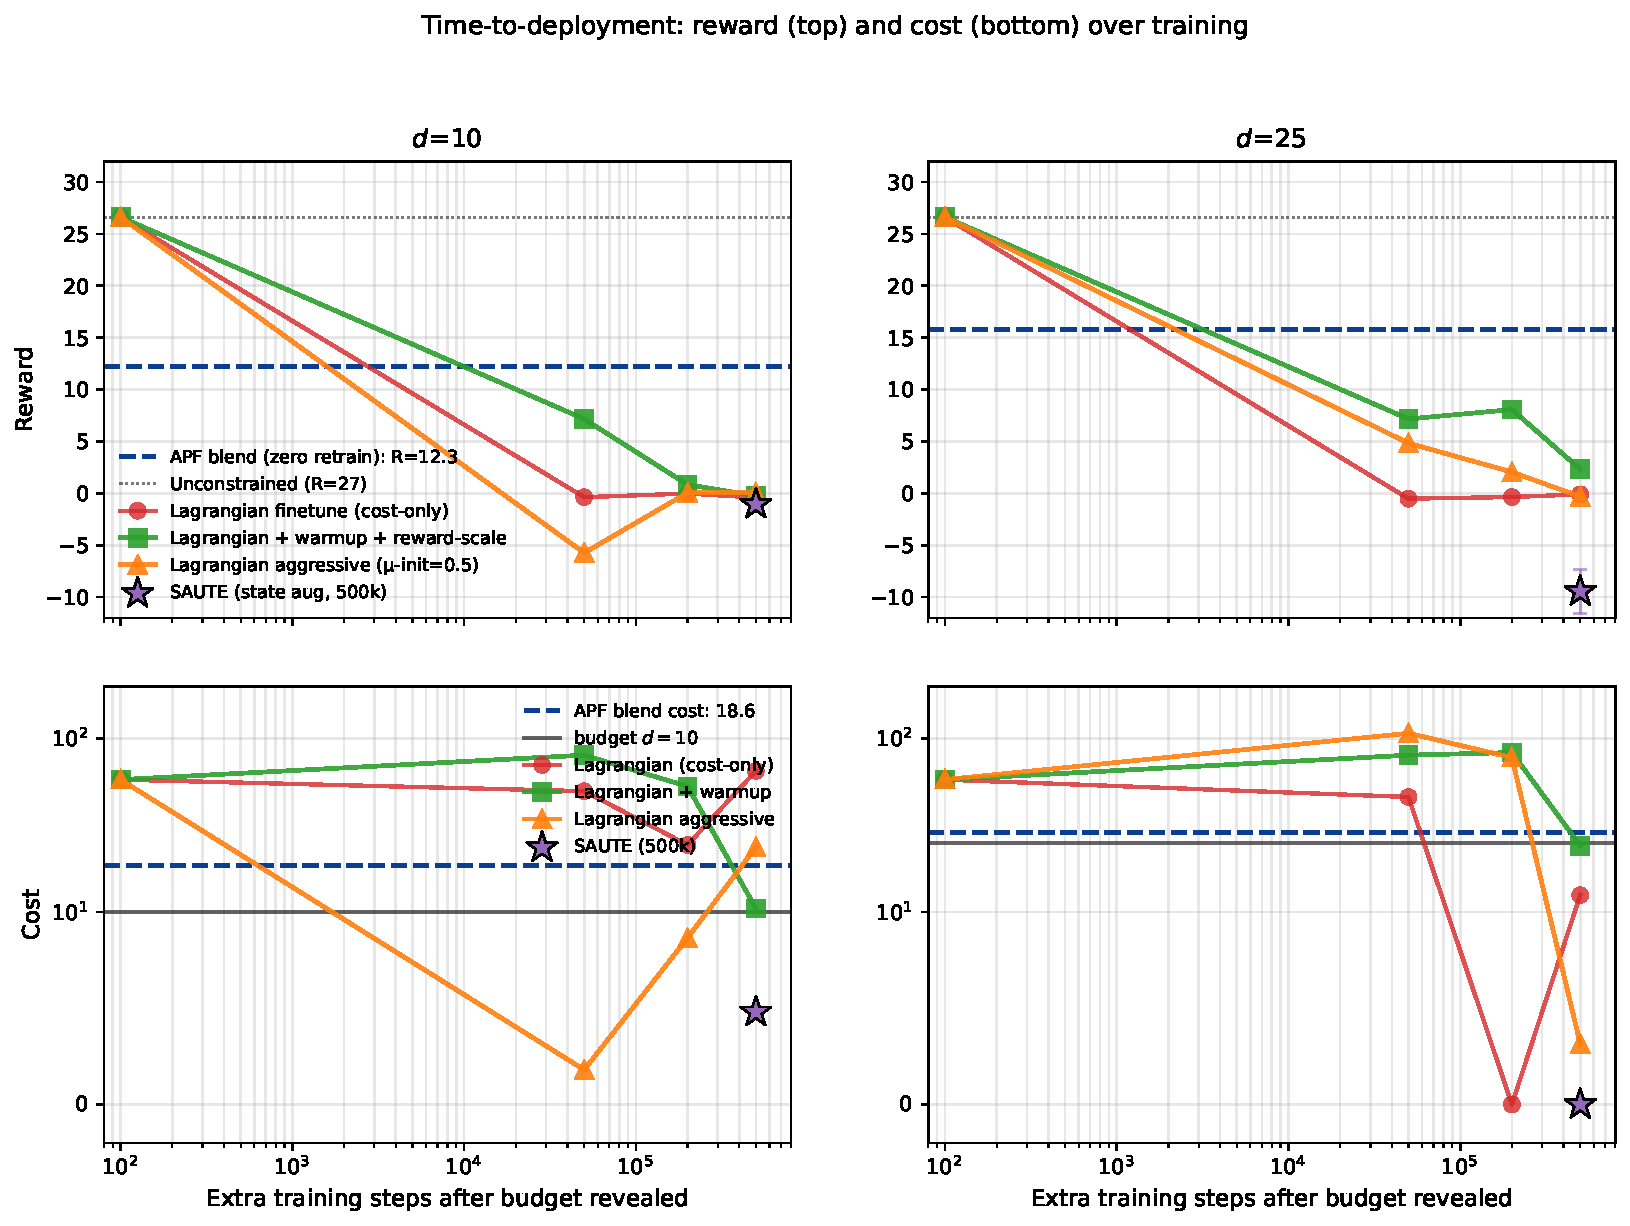
\includegraphics[width=\linewidth]{figures/fig_time_to_deployment.pdf}
    \caption{Time-to-deployment on Safety Gymnasium PointGoal1, both budgets and both axes. \emph{Top row}: reward over extra training steps. \emph{Bottom row}: cost over the same axis with budget line. Blue dashed: APF-blend reward and cost at zero retraining. Curves: four CMDP retraining variants starting from the same pretrained actor (single seed each, four hyperparameter regimes); star: SAUTE~\citep{sootla2022saute} at 500k. The blend retains higher reward than every retraining variant tested at every checkpoint, but its cost (18.6 at $d\!=\!10$, 28.6 at $d\!=\!25$) exceeds the budget; some retraining variants satisfy the budget tightly at the price of $R\!\approx\!0$. The two methods occupy different points on the reward-cost frontier.}
    \label{fig:time_to_deployment}
\end{figure}

\begin{table}[h]
\centering
\caption{Final-step ($500$k) baseline summary on Safety Gymnasium. \textbf{$\mathbb{E}[C]\!\le\!d$}: expected-cost feasibility. The APF blend dominates the retraining baselines \emph{on the reward axis} at the same compute budget. Some retraining baselines satisfy the cost constraint more tightly at the price of near-zero reward.}
\label{tab:baselines}
\begin{tabular}{lcccc}
\toprule
Method & $d$ & Reward & Cost & $\mathbb{E}[C]\!\le\!d$ \\
\midrule
\textbf{APF blend (zero retraining)} & 10 & $\mathbf{12.3}$ & $18.6$ & \textcolor{red}{$\times$} \\
\textbf{APF blend (zero retraining)} & 25 & $\mathbf{15.8}$ & $28.6$ & \textcolor{red}{$\times$} \\
\midrule
SAC-Lag default                      & 10 & $-0.41$ & $65.0$ & \textcolor{red}{$\times$} \\
SAC-Lag default                      & 25 & $-0.10$ & $12.5$ & \checkmark \\
SAC-Lag warmup + reward-scale        & 10 & $-0.24$ & $10.4$ & \textcolor{red}{$\times$} \\
SAC-Lag warmup + reward-scale        & 25 & $2.32$  & $24.1$ & \checkmark \\
SAC-Lag aggressive                   & 10 & $0.07$  & $23.6$ & \textcolor{red}{$\times$} \\
SAC-Lag aggressive                   & 25 & $-0.32$ & $3.1$  & \checkmark \\
SAUTE (state aug, uses $\rho_t$)     & 10 & $-1.0$  & $4.8$  & \checkmark \\
SAUTE (state aug, uses $\rho_t$)     & 25 & $-9.5$  & $0.0$  & \checkmark \\
\bottomrule
\end{tabular}
\end{table}

Two distinct operating regimes appear.
The post-hoc blend gives the highest reward at every compute checkpoint but violates the cost constraint in expectation at $d\!\in\!\{10, 25\}$ (it is feasible at $d\!=\!40$, Table~\ref{tab:safetygym}).
Retraining baselines either violate the budget while preserving partial reward (warmup at intermediate checkpoints) or satisfy it by collapsing reward to $\approx\!0$ (aggressive Lagrangian, SAUTE).
\textbf{Neither method dominates in the strict constrained-optimisation sense; they occupy different points on the reward-cost frontier.}
A practitioner should choose based on whether their constraint is operationally a soft pacing target (favour the blend, retain useful policy) or a hard expected-cost limit (favour SAC-Lag warmup or SAUTE, accept reward collapse).
We do not claim retraining cannot eventually reach better operating points with more compute; under the budgets we tested, the blend offers a competitive position on the reward axis with zero retraining.
